\documentclass[]{book}
\usepackage{lmodern}
\usepackage{amssymb,amsmath}
\usepackage{ifxetex,ifluatex}
\usepackage{fixltx2e} % provides \textsubscript
\ifnum 0\ifxetex 1\fi\ifluatex 1\fi=0 % if pdftex
  \usepackage[T1]{fontenc}
  \usepackage[utf8]{inputenc}
\else % if luatex or xelatex
  \ifxetex
    \usepackage{mathspec}
  \else
    \usepackage{fontspec}
  \fi
  \defaultfontfeatures{Ligatures=TeX,Scale=MatchLowercase}
\fi
% use upquote if available, for straight quotes in verbatim environments
\IfFileExists{upquote.sty}{\usepackage{upquote}}{}
% use microtype if available
\IfFileExists{microtype.sty}{%
\usepackage{microtype}
\UseMicrotypeSet[protrusion]{basicmath} % disable protrusion for tt fonts
}{}
\usepackage[margin=1in]{geometry}
\usepackage{hyperref}
\hypersetup{unicode=true,
            pdftitle={Machine Learning},
            pdfauthor={Mohamad Ghassany},
            pdfborder={0 0 0},
            breaklinks=true}
\urlstyle{same}  % don't use monospace font for urls
\usepackage{natbib}
\bibliographystyle{apalike}
\usepackage{longtable,booktabs}
\usepackage{graphicx,grffile}
\makeatletter
\def\maxwidth{\ifdim\Gin@nat@width>\linewidth\linewidth\else\Gin@nat@width\fi}
\def\maxheight{\ifdim\Gin@nat@height>\textheight\textheight\else\Gin@nat@height\fi}
\makeatother
% Scale images if necessary, so that they will not overflow the page
% margins by default, and it is still possible to overwrite the defaults
% using explicit options in \includegraphics[width, height, ...]{}
\setkeys{Gin}{width=\maxwidth,height=\maxheight,keepaspectratio}
\IfFileExists{parskip.sty}{%
\usepackage{parskip}
}{% else
\setlength{\parindent}{0pt}
\setlength{\parskip}{6pt plus 2pt minus 1pt}
}
\setlength{\emergencystretch}{3em}  % prevent overfull lines
\providecommand{\tightlist}{%
  \setlength{\itemsep}{0pt}\setlength{\parskip}{0pt}}
\setcounter{secnumdepth}{5}
% Redefines (sub)paragraphs to behave more like sections
\ifx\paragraph\undefined\else
\let\oldparagraph\paragraph
\renewcommand{\paragraph}[1]{\oldparagraph{#1}\mbox{}}
\fi
\ifx\subparagraph\undefined\else
\let\oldsubparagraph\subparagraph
\renewcommand{\subparagraph}[1]{\oldsubparagraph{#1}\mbox{}}
\fi

%%% Use protect on footnotes to avoid problems with footnotes in titles
\let\rmarkdownfootnote\footnote%
\def\footnote{\protect\rmarkdownfootnote}

%%% Change title format to be more compact
\usepackage{titling}

% Create subtitle command for use in maketitle
\newcommand{\subtitle}[1]{
  \posttitle{
    \begin{center}\large#1\end{center}
    }
}

\setlength{\droptitle}{-2em}
  \title{Machine Learning}
  \pretitle{\vspace{\droptitle}\centering\huge}
  \posttitle{\par}
  \author{Mohamad Ghassany}
  \preauthor{\centering\large\emph}
  \postauthor{\par}
  \predate{\centering\large\emph}
  \postdate{\par}
  \date{2018-01-11}

% \defaultfontfeatures{
%     Path = /home/ghassany/texmf/fonts/opentype/public/fontawesome/}
\usepackage{fontawesome}

\usepackage{booktabs}
\usepackage{longtable}
\usepackage{framed,color}
\usepackage{float}
\let\origfigure\figure
\let\endorigfigure\endfigure
\renewenvironment{figure}[1][2] {
    \expandafter\origfigure\expandafter[H]
} {
    \endorigfigure
}

\definecolor{shadecolor}{RGB}{248,248,248}

\ifxetex
  \usepackage{letltxmacro}
  \setlength{\XeTeXLinkMargin}{1pt}
  \LetLtxMacro\SavedIncludeGraphics\includegraphics
  \def\includegraphics#1#{% #1 catches optional stuff (star/opt. arg.)
    \IncludeGraphicsAux{#1}%
  }%
  \newcommand*{\IncludeGraphicsAux}[2]{%
    \XeTeXLinkBox{%
      \SavedIncludeGraphics#1{#2}%
    }%
  }%
\fi

\newenvironment{rmdblock}[1]
  {\begin{shaded*}
  \begin{itemize}
  \renewcommand{\labelitemi}{
    \raisebox{-.7\height}[0pt][0pt]{
      {\setkeys{Gin}{width=2em,keepaspectratio}\includegraphics{img/icons/#1}}
    }
  }
  \item
  }
  {
  \end{itemize}
  \end{shaded*}
  }
\newenvironment{rmdcaution}
  {\begin{rmdblock}{caution}}
  {\end{rmdblock}}
\newenvironment{rmdinsight}
  {\begin{rmdblock}{insight}}
  {\end{rmdblock}}
\newenvironment{rmdexercise}
  {\begin{rmdblock}{exercise}}
  {\end{rmdblock}}
\newenvironment{rmdtip}
  {\begin{rmdblock}{tip}}
  {\end{rmdblock}}
\newenvironment{rmdnoicon}
  {\begin{rmdblock}}
  {\end{rmdblock}}

\usepackage{amsthm}
\newtheorem{theorem}{Theorem}[chapter]
\newtheorem{lemma}{Lemma}[chapter]
\theoremstyle{definition}
\newtheorem{definition}{Definition}[chapter]
\newtheorem{corollary}{Corollary}[chapter]
\newtheorem{proposition}{Proposition}[chapter]
\theoremstyle{definition}
\newtheorem{example}{Example}[chapter]
\theoremstyle{definition}
\newtheorem{exercise}{Exercise}[chapter]
\theoremstyle{remark}
\newtheorem*{remark}{Remark}
\newtheorem*{solution}{Solution}
\begin{document}
\maketitle

{
\setcounter{tocdepth}{2}
\tableofcontents
}
\chapter*{Welcome}\label{welcome}
\addcontentsline{toc}{chapter}{Welcome}

Welcome to this course. It is only a little introduction to Machine
Learning.

The aim of Machine Learning is to build computer systems that can adapt
to their environments and learn form experience. Learning techniques and
methods from this field are successfully applied to a variety of
learning tasks in a broad range of areas, including, for example, spam
recognition, text classification, gene discovery, financial forecasting.
The course will give an overview of many concepts, techniques, and
algorithms in machine learning, beginning with topics such as linear
regression and classification and ending up with topics such as kmeans
and Expectation Maximization. The course will give the student the basic
ideas and intuition behind these methods, as well as a more formal
statistical and computational understanding. Students will have an
opportunity to experiment with machine learning techniques in R and
apply them to a selected problem.

\section*{Course Overview}\label{course-overview}
\addcontentsline{toc}{section}{Course Overview}

\chapter*{Introduction}\label{introduction}
\addcontentsline{toc}{chapter}{Introduction}

\section*{What is Machine Learning ?}\label{what-is-machine-learning}
\addcontentsline{toc}{section}{What is Machine Learning ?}

What is Machine Learning?

Two definitions of Machine Learning are offered. Arthur Samuel described
it as: ``the field of study that gives computers the ability to learn
without being explicitly programmed.'' This is an older, informal
definition.

Tom Mitchell provides a more modern definition: ``A computer program is
said to learn from experience E with respect to some class of tasks T
and performance measure P, if its performance at tasks in T, as measured
by P, improves with experience E.''

Machine Learning is also called Statistical Learning.

Example: playing checkers.

E = the experience of playing many games of checkers

T = the task of playing checkers.

P = the probability that the program will win the next game.

In general, any machine learning problem can be assigned to one of two
broad classifications:

Supervised learning and Unsupervised learning.

\section*{Supervised Learning}\label{supervised-learning}
\addcontentsline{toc}{section}{Supervised Learning}

Supervised Learning is probably the most common type of machine learning
problem. Let's start with an example of what is it. Let's say we want to
predict housing prices. We plot a data set and it looks like this.

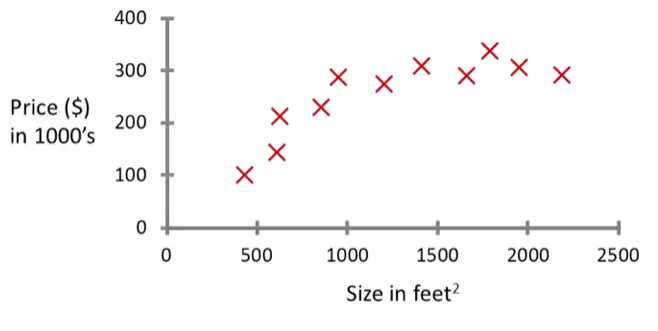
\includegraphics{img/sl1.png}

Here on the horizontal axis, the size of different houses in square
feet, and on the vertical axis, the price of different houses in
thousands of dollars.

So. Given this data, let's say we own a house that is, say 750 square
feet and hoping to sell the house and we want to know how much we can
get for the house.

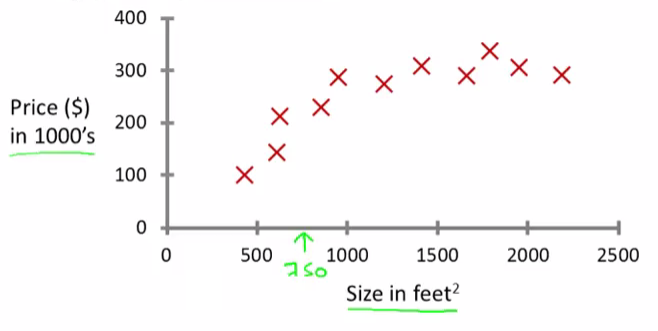
\includegraphics{img/sl2.png}

So how can the learning algorithm help?

One thing a learning algorithm might be able to do is put a straight
line through the data or to \textbf{``fit''} a straight line to the data
and, based on that, it looks like maybe the house can be sold for maybe
about \$150,000.

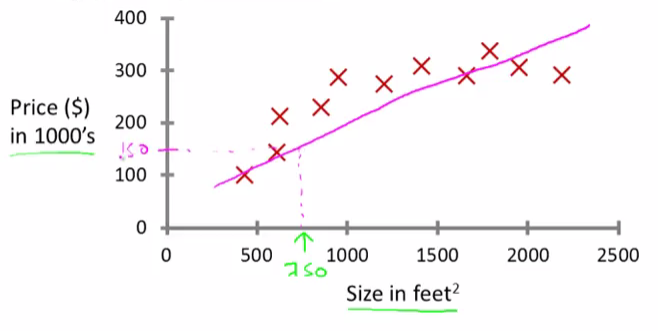
\includegraphics{img/sl3.png}

But maybe this isn't the only learning algorithm we can use. There might
be a better one. For example, instead of sending a straight line to the
data, we might decide that it's better to fit a \emph{quadratic
function} or a \emph{second-order polynomial} to this data.

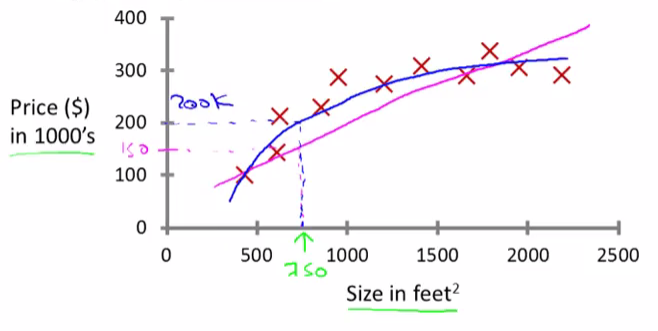
\includegraphics{img/sl4.png}

If we do that, and make a prediction here, then it looks like, well,
maybe we can sell the house for closer to \$200,000.

This is an example of a supervised learning algorithm.

The term supervised learning refers to the fact that we gave the
algorithm a data set in which the \textbf{``right answers''} were given.

The example above is also called a regression problem. A regression
problem is when we try to predict a \textbf{continuous} value output.
Namely the price in the example.

Here's another supervised learning example. Let's say we want to look at
medical records and try to predict of a breast cancer as malignant or
benign. If someone discovers a breast tumor, a lump in their breast, a
malignant tumor is a tumor that is harmful and dangerous and a benign
tumor is a tumor that is harmless. Let's see a collected data set and
suppose in the data set we have the size of the tumor on the horizontal
axis and on the vertical axis we plot one or zero, yes or no, whether or
not these are examples of tumors we've seen before are malignant (which
is one) or zero if not malignant or benign.

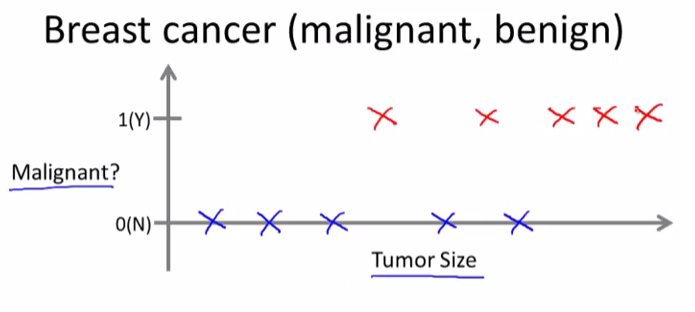
\includegraphics{img/sl5.png}

In this data set we have five examples of benign tumors, and five
examples of malignant tumors.

Let's say a person who tragically has a breast tumor, and let's say her
breast tumor size is known (rose arrow in the following figure).

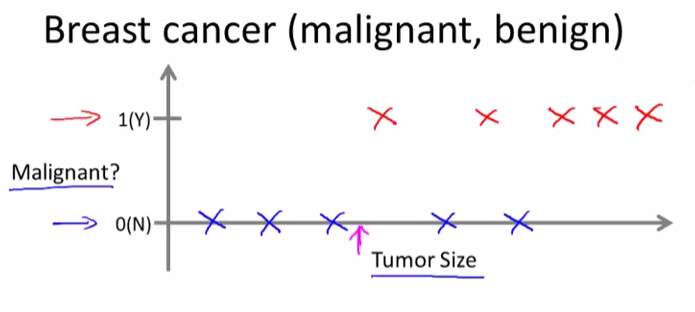
\includegraphics{img/sl6.png}

The machine learning question is, can you estimate what is the
probability that a tumor is malignant versus benign? To introduce a bit
more terminology this is an example of a \textbf{\emph{classification}}
problem.

The term classification refers to the fact that here we're trying to
predict a \textbf{discrete} value output: zero or one, malignant or
benign. And it turns out that in classification problems sometimes you
can have more than two values for the two possible values for the
output.

In classification problems there is another way to plot this data. Let's
use a slightly different set of symbols to plot this data. So if tumor
size is going to be the attribute that we are going to use to predict
malignancy or benignness, we can also draw the data like this.

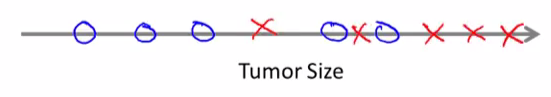
\includegraphics{img/sl7.png}

All we did was we took the data set on top and just mapped it down using
different symbols. So instead of drawing crosses, we are now going to
draw \texttt{O}'s for the benign tumors.

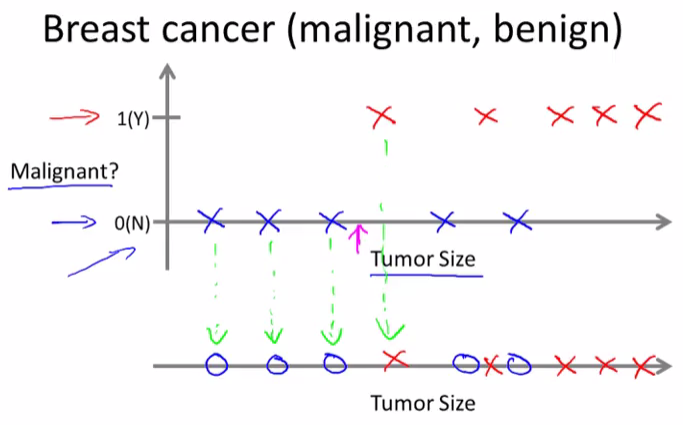
\includegraphics{img/sl8.png}

Now, in this example we use only one \textbf{feature} or one attribute,
mainly, the \emph{tumor size} in order to predict whether the tumor is
malignant or benign.

In other machine learning problems we may have more than one feature.

Here's an example. Let's say that instead of just knowing the tumor
size, we know both the age of the patients and the tumor size. In that
case maybe the data set will look like this.

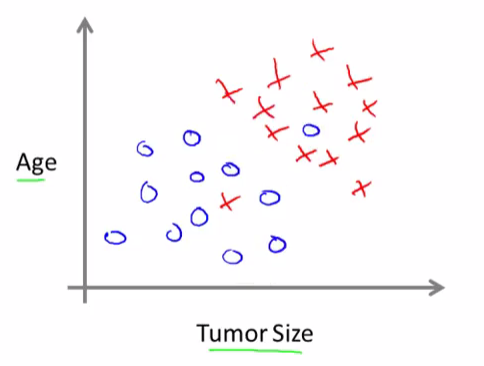
\includegraphics{img/sl9.png}

So, let's say a person who tragically has a tumor. And maybe, their
tumor size and age falls around there (rose point):

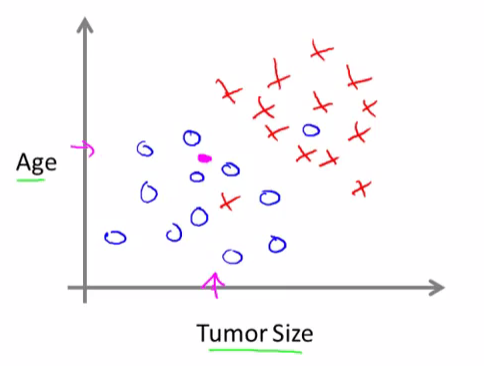
\includegraphics{img/sl10.png}

So given a data set like this, what the learning algorithm might do is
throw a straight line through the data to try to separate out the
malignant tumors from the benign ones. And with this, hopefully we can
decide that the person's tumor falls on this benign side and is
therefore more likely to be benign than malignant.

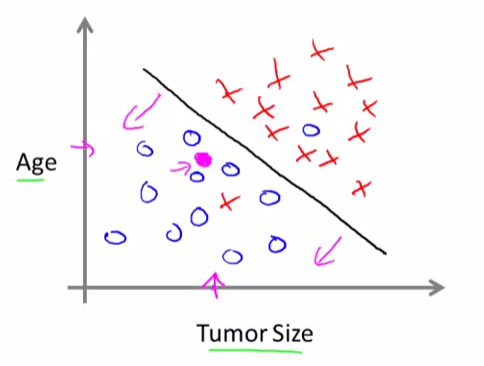
\includegraphics{img/sl11.png}

In this example we had \textbf{two features}, namely, the age of the
patient and the size of the tumor. In other machine learning problems we
will often have more features.

Most interesting learning algorithms is a learning algorithm that can
deal with, not just two or three or five features, but an
\textbf{infinite number of features}. So how do you deal with an
infinite number of features. How do you even store an infinite number of
things on the computer when your computer is gonna run out of memory.

\section*{Unsupervised Learning}\label{unsupervised-learning}
\addcontentsline{toc}{section}{Unsupervised Learning}

The second major type of machine learning problem is called Unsupervised
Learning.

The difference between Unsupervised Learning and Supervised Learning is
that in Supervised Learning we are told explicitly what is the so-called
right answers (data are labeled).

In Unsupervised Learning, we're given data that doesn't have any labels
or that all has the same label or really no labels. Like in this
example:

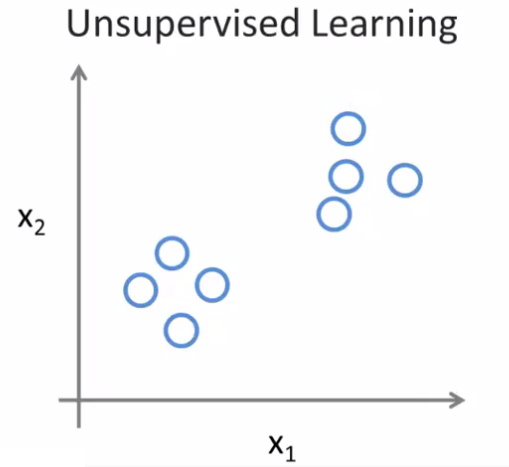
\includegraphics{img/ul1.png}

So we're given the data set and we're not told what to do with it and
we're not told what each data point is. Instead we're just told, here is
a data set. Can you find some structure in the data?

Given this data set, an Unsupervised Learning algorithm might decide
that the data lives in two different clusters.

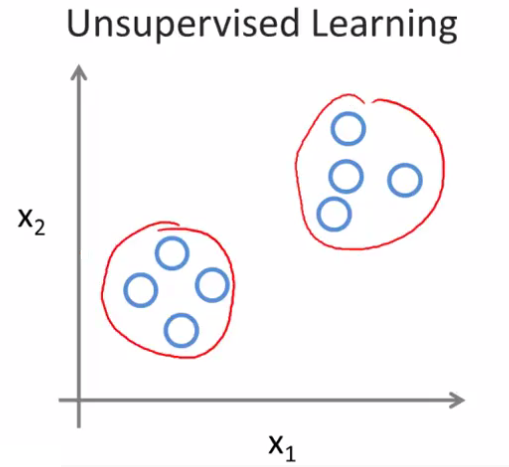
\includegraphics{img/ul2.png}

This is called a \textbf{clustering} algorithm.

Here are two examples where Unsupervised Learning or clustering is used.

Social network analysis:

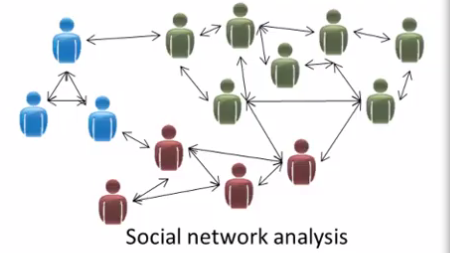
\includegraphics{img/ul3.png}

So given knowledge about which friends you email the most or given your
Facebook friends or your Google+ circles, can we automatically identify
which are cohesive groups of friends, also which are groups of people
that all know each other?

Market segmentation:

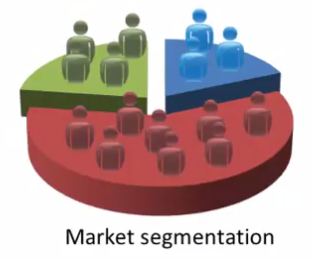
\includegraphics{img/ul4.png}

Many companies have huge databases of customer information. So, can you
look at this customer data set and automatically discover market
segments and automatically group your customers into different market
segments so that you can automatically and more efficiently sell or
market your different market segments together?

This is Unsupervised Learning because we have all this customer data,
but we don't know in advance what are the market segments and for the
customers in our data set, we don't know in advance who is in market
segment one, who is in market segment two, and so on. But we have to let
the algorithm discover all this just from the data.

◼

\part{Supervised Learning}\label{part-supervised-learning}

\chapter{Linear Regression}\label{linear-regression}

\section{Notation}\label{notation}

In general, we will let \(x_{ij}\) represent the value of the \(j\)th
variable for the \(i\)th observation, where \(i=1,2,\ldots,n\) and
\(j=1,2,\ldots,p\). We will use \(i\) to index the samples or
observations (from \(1\) tp \(n\)) and \(j\) will be used to index the
variables (or features) (from \(1\) to \(p\)). We let \(\textbf{X}\)
denote a \(n \times p\) matrix whose \((i,j)\)th element is \(x_{ij}\).
That is,

\[ \textbf{X}  = \begin{pmatrix}
    x_{11} & x_{12} & x_{13} & \dots  & x_{1p} \\
    x_{21} & x_{22} & x_{23} & \dots  & x_{2p} \\
    \vdots & \vdots & \vdots & \ddots & \vdots \\
    x_{n1} & x_{n2} & x_{n3} & \dots  & x_{np}
\end{pmatrix} \]

Note that it is useful to visualize \(\textbf{X}\) as a spreadsheet of
numbers with \(n\) rows and \(p\) columns. We will write the rows of
\(\textbf{X}\) as \(x_1 , x_2 , \ldots, x_n\). Here \(x_i\) is a vector
of length \(p\), containing the \(p\) variable measurements for the
\(i\)th observation. That is,

\[ x_i = \begin{pmatrix}
    x_{i1} \\
    x_{i2} \\
    \vdots \\
    x_{ip}
\end{pmatrix}\]

(Vectors are by default represented as columns.)

We will write the columns of \(\textbf{X}\) as
\(\textbf{x}_1 , \textbf{x}_2, \ldots, \textbf{x}_p\). Each is a vector
of length \(n\). That is,

\[ \textbf{x}_j = \begin{pmatrix}
    \textbf{x}_{1j} \\
    \textbf{x}_{2j} \\
    \vdots \\
    \textbf{x}_{nj}
\end{pmatrix}\]

Using this notation, the matrix \(\textbf{X}\) can be written as

\[ \textbf{X} = (\textbf{x}_1  \textbf{x}_2 \ldots \textbf{x}_p) \]

or

\[ \textbf{X} = \begin{pmatrix}
    x_{1}^T \\
    x_{2}^T \\
    \vdots \\
    x_{n}^T
\end{pmatrix}\]

The \(^T\) notation denotes the transpose of a matrix or vector.

We use \(y_i\) to denote the \(i\)th observation of the variable on
which we wish to make predictions. We write the set of all \(n\)
observations in vector form as

\[ \textbf{y} = \begin{pmatrix}
    y_{1}^T \\
    y_{2}^T \\
    \vdots \\
    y_{n}^T
\end{pmatrix}\]

Then the observed data consists of
\(\{(x_1, y_1), (x_2 , y_2 ), \ldots , (x_n , y_n )\}\), where each
\(x_i\) is a vector of length \(p\). (If \(p = 1\), then \(x_i\) is
simply a scalar).

\section{Model Representation}\label{model-representation}

Let's consider the example about predicting housing prices. We're going
to use this data set as an example,

\begin{figure}
\centering
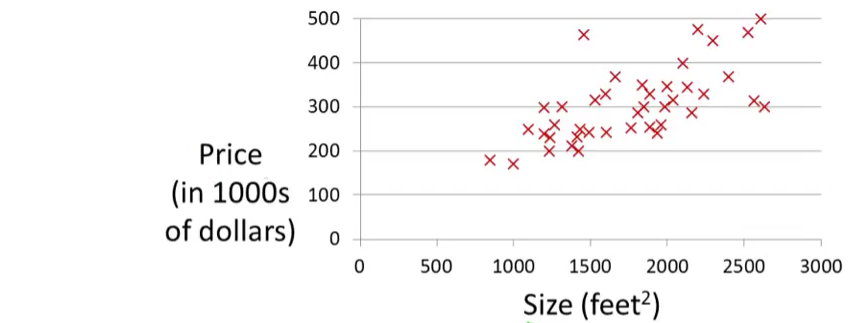
\includegraphics{img/mr1.png}
\caption{}
\end{figure}

Suppose that there is a person trying to sell a house of size 1250
square feet and he wants to know how much he might be able to sell the
house for. One thing we could do is fit a model. Maybe fit a straight
line to this data. Looks something like this,

\begin{figure}
\centering
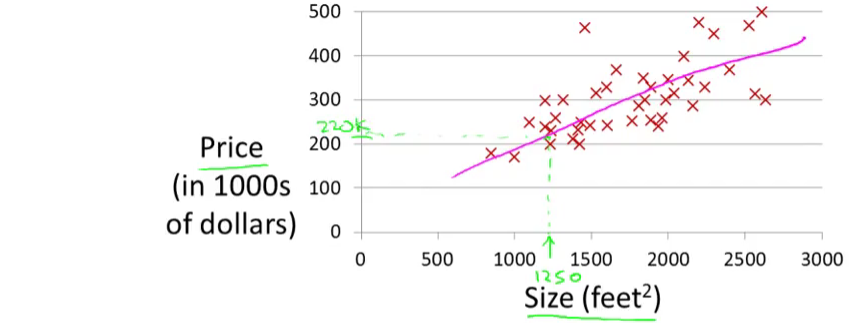
\includegraphics{img/mr2.png}
\caption{}
\end{figure}

and based on that, maybe he can sell the house for around \$220,000.
Recall that this is an example of a supervised learning algorithm. And
it's supervised learning because we're given the ``right answer'' for
each of our examples. More precisely, this is an example of a regression
problem where the term regression refers to the fact that we are
predicting a real-valued output namely the price.

More formally, in supervised learning, we have a data set and this data
set is called a \textbf{training set}. So for housing prices example, we
have a training set of different housing prices and our job is to learn
from this data how to predict prices of the houses.

Let's define some notation from this data set:

\begin{itemize}
\tightlist
\item
  The size of the house is the input variable.
\item
  The house price is the output variable.
\item
  The input variables are typically denoted using the variable symbol
  \(X\),
\item
  The inputs go by different names, such as \emph{predictors},
  \emph{independent variables}, \emph{features}, \emph{predictor} or
  sometimes just \emph{variables}.
\item
  The output variable is often called the \emph{response},
  \emph{dependent variable} or \emph{target}, and is typically denoted
  using the symbol \(Y\).
\item
  \((x_i,y_i)\) is the \(i\)th training example.
\item
  The set of \(\{(x_i, y_i)\}\) is the training set.
\item
  \(n\) is the number of training examples.
\end{itemize}

So here's how this supervised learning algorithm works. Suppose that we
observe a quantitative response \(Y\) and \(p\) different predictors,
\(X_1 , X_2 ,\ldots, X_p\) . We assume that there is some relationship
between \(Y\) and \(X = (X_1 , X_2 ,\ldots, X_p)\), which can be written
in the very general form

\[Y = f(X) + \epsilon\]

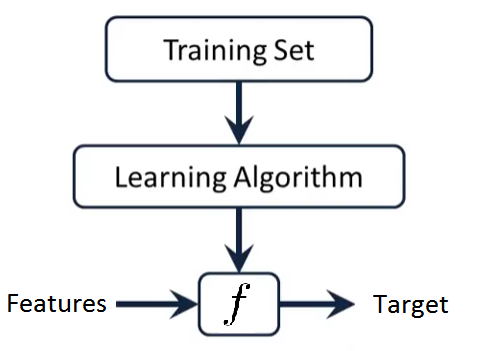
\includegraphics{img/mr3.png}

Here \(f\) is some fixed but unknown function of
\(X_1 , X_2 ,\ldots, X_p\) , and \(\epsilon\) is a random error term,
which is independent of \(X\) and has mean zero. The \(f\) function is
also called \emph{hypothesis} in Machine Learning. In general, the
function \(f\) may involve more than one input variable. In essence,
Supervised Learning refers to a set of approaches for estimating \(f\).

\section{\texorpdfstring{Why Estimate \(f\)
?}{Why Estimate f ?}}\label{why-estimate-f}

There are two main reasons that we may wish to estimate \(f\):
\emph{prediction} and \emph{inference}.

\subsection*{Prediction}\label{prediction}
\addcontentsline{toc}{subsection}{Prediction}

In many situations, a set of inputs \(X\) are readily available, but the
output \(Y\) cannot be easily obtained. In this setting, since the error
term averages to zero, we can predict \(Y\) using

\[ \hat{Y} = \hat{f}(X) \]

where \(\hat{f}\) represents our estimate for \(f\), and \(\hat{Y}\)
represents the resulting prediction for \(Y\). Like in the example above
about predicting housing prices.

We can measure the accuracy of \(\hat{Y}\) by using a \textbf{cost
function}. In the regression models, the most commonly-used measure is
the \emph{mean squared error} (MSE), given by

\[ MSE = \frac{1}{n} \sum_{i=1}^{n} (y_i - \hat{f}(x_i))^2\]

\subsection*{Inference}\label{inference}
\addcontentsline{toc}{subsection}{Inference}

We are often interested in understanding the way that \(Y\) is affected
as \(X_1 , X_2 ,\ldots, X_p\) change. In this situation we wish to
estimate \(f\) , but our goal is not necessarily to make predictions for
\(Y\). We instead want to understand the relationship between \(X\) and
\(Y\), or more specifically, to understand how \(Y\) changes as a
function of \(X_1 , X_2 ,\ldots, X_p\). In this case, one may be
interested in answering the following questions:

\begin{itemize}
\tightlist
\item
  Which predictors are associated with the response?
\item
  What is the relationship between the response and each predictor?
\item
  Can the relationship between Y and each predictor be adequately
  summarized using a linear equation, or is the relationship more
  complicated?
\end{itemize}

\section{Simple Linear Regression
Model}\label{simple-linear-regression-model}

\emph{Simple linear regression} is a very straightforward approach for
predicting a quantitative response \(Y\) on the basis of a single
predictor variable \(X\). It assumes that there is approximately a
linear relationship between \(X\) and \(Y\). Mathematically, we can
write this linear relationship as

\[ Y = \beta_0 + \beta_1 X + \epsilon \]
\[Y \approx \beta_0 + \beta_1 X\]

where \(\beta_0\) and \(\beta_1\) are two unknown constants that
represent the \emph{intercept} and \emph{slope}, also known as
\textbf{\emph{coefficients}} or \emph{parameters}, and \(\epsilon\) is
the error term.

Given some estimates \(\hat{\beta_0}\) and \(\hat{\beta_1}\) for the
model coefficients, we predict future inputs \(x\) using

\[\hat{y} = \hat{\beta_0} + \hat{\beta_1} x\]

where \(\hat{y}\) indicates a prediction of \(Y\) on the basis of
\(X = x\). The \emph{hat} symbol, \(\hat{}\), denotes an estimated
value.

\section{Estimating the Coefficients}\label{estimating-the-coefficients}

Let \(\hat{y}_i = \hat{\beta_0} + \hat{\beta_1} x_i\) be the prediction
for \(Y\) based on the \(i\)th value of \(X\). Then
\(e_i = y_i - \hat{y}_i\) represents the \(i\)th
\textbf{\emph{residual}}.

We define the \textbf{\emph{residual sum of squares}} (\textbf{RSS}) as

\[  \begin{aligned}
RSS &= e_1^2 + e_2^2 + \ldots + e_n^2 \\
    &= \sum_{i=1}^{n} e_i^2
 \end{aligned}  \]

or equivantly as

\[ \begin{aligned}
RSS &= (y_1 - \hat{\beta_0} - \hat{\beta_1} x_1)^2 + (y_2 - \hat{\beta_0} - \hat{\beta_1} x_2)^2 + \ldots + (y_n - \hat{\beta_0} - \hat{\beta_1} x_n)^2 \\
    &= \sum_{i=1}^{n} (y_i - \hat{\beta_0} - \hat{\beta_1} x_i)^2
\end{aligned} \]

The \emph{least squares} approach chooses \(\hat{\beta_0}\) and
\(\hat{\beta_1}\) to minimize the RSS. The minimizing values can be show
to be

\[  \begin{aligned}
\hat{\beta_1} &=  \frac{\sum_{i=1}^{n} (x_i - \bar{x})(y_i - \bar{y})  }{\sum_{i=1}^{n} (x_i - \bar{x})^2 } = \frac{s_{xy}}{s_x^2} \\
\text{and} \\
\hat{\beta_0} &= \bar{y} - \hat{\beta_1} \bar{x}
\end{aligned}  \]

where:

\begin{itemize}
\tightlist
\item
  \(\bar{x}=\frac{1}{n}\sum_{i=1}^nx_i\) is the \emph{sample mean}.
\item
  \(s_x^2=\frac{1}{n}\sum_{i=1}^n(x_i-\bar{x})^2\) is the \emph{sample
  variance}. The sample standard deviation is \(s_x=\sqrt{s_x^2}\).
\item
  \(s_{xy}=\frac{1}{n}\sum_{i=1}^n(x_i-\bar{x})(y_i-\bar{y})\) is the
  \emph{sample covariance}. It measures the degree of linear association
  between \(x_1,\ldots,x_n\) and \(y_1,\ldots,y_n\). Once scaled by
  \(s_xs_y\), it gives the \emph{sample correlation coefficient},
  \(r_{xy}=\frac{s_{xy}}{s_xs_y}\).
\end{itemize}

\begin{rmdinsight}
Click here to see the influence of the distance employed in the sum of
squares. Try to minimize the sum of squares for the different datasets.
The choices of intercept and slope that minimize the sum of squared
distances for a kind of distance are not the optimal for a different
kind of distance.
\end{rmdinsight}

\section{Assessing the Accuracy of the Coefficient
Estimates}\label{assessing-the-accuracy-of-the-coefficient-estimates}

The standard error of an estimator reflects how it varies under repeated
sampling. We have

\[ \text{SE}(\hat{\beta_1})^2 =  \frac{\sigma^2}{\sum_{i=1}^{n} (x_i - \bar{x})^2} \]

\[ \text{SE}(\hat{\beta_0})^2 = \sigma^2 \bigg[ \frac{1}{n} +  \frac{\bar{x}^2}{\sum_{i=1}^{n} (x_i - \bar{x})^2} \bigg] \]

where \(\sigma^2 = Var(\epsilon)\)

In general, \(\sigma^2\) is unknown, but can be estimated from the data.
The estimate of \(\sigma\) is known as the \emph{residual standard
error}, and is given by

\[ \text{RSE} = \sqrt{\frac{\text{RSS}}{(n-2)}} \]

These standard errors can be used to compute \emph{confidence
intervals}. A \(95\%\) confidence interval is defined as a range of
values such that with \(95\%\) probability, the range will contain the
true unknown value of the parameter. It has the form

\[ \hat{\beta_1} \pm 2 \cdot \text{SE}(\hat{\beta_1}) \]

That is, there is approximately a \(95\%\) chance that the interval

\[ \bigg[  \hat{\beta_1} - 2 \cdot \text{SE}(\hat{\beta_1}), \hat{\beta_1} + 2 \cdot \text{SE}(\hat{\beta_1})   \bigg] \]

will contain the true value of \(\beta_1\). Similarly, a confidence
interval for \(\beta_0\) approximately takes the form

\[ \hat{\beta_0} \pm 2 \cdot \text{SE}(\hat{\beta_0}) \]

\subsection*{Hypothesis testing}\label{hypothesis-testing}
\addcontentsline{toc}{subsection}{Hypothesis testing}

Standard errors can also be used to perform \emph{hypothesis tests} on
the coefficients. The most common hypothesis test involves testing the
\emph{null hypothesis} of

\[ H_0 : \text{There is no relationship between} \, X \, \text{and} \, Y \]

versus the \emph{alternative hypothesis}

\[ H_1 : \text{There is some relationship between} \, X \, \text{and} \, Y \]

Mathematically, this corresponds to testing

\[ H_0 : \beta_1 = 0 \]

versus

\[ H_1 : \beta_1 \neq 0 \]

since if \(\beta_1 = 0\) then the simple linear regression model reduces
to \(Y = \beta_0 + \epsilon\), and \(X\) is not associated with \(Y\).

To test the null hypothesis \(H_0\), we compute a
\textbf{\emph{t-statistic}}, given by

\[ t = \frac{\hat{\beta_1} - 0}{\text{SE}(\hat{\beta_1})} \]

This will have a \(t\)-distribution (\emph{Student}) with \(n-2\)
degrees of freedom, assuming \(\beta_1=0\).

Using statistical software, it is easy to compute the probability of
observing any value equal to \(|t|\) or larger. We call this probability
the \textbf{\emph{p-value}}.

If p-value is small enough (typically under \(0.01\) (\(1\%\) error) or
\(0.05\) (\(5\%\) error)) we reject the null hypothesis, that is we
declare a relationship to exist between \(X\) and \(Y\).

\section{ANOVA and model fit}\label{anova-and-model-fit}

\subsection{ANOVA}\label{anova}

In this section we will see how the variance of \(Y\) is decomposed into
two parts, each one corresponding to the regression and to the error,
respectively. This decomposition is called the \emph{ANalysis Of
VAriance} (ANOVA).

Before explaining ANOVA, it is important to recall an interesting
result: \emph{the mean of the fitted values \(\hat Y_1,\ldots,\hat Y_n\)
is the mean of \(Y_1,\ldots, Y_n\)}. This is easily seen if we plug-in
the expression of \(\hat\beta_0\):

\begin{align*}
\frac{1}{n}\sum_{i=1}^n \hat Y_i=\frac{1}{n}\sum_{i=1}^n \left(\hat \beta_0+\hat\beta_1X_i\right)=\hat \beta_0+\hat\beta_1\bar X=\left(\bar Y - \hat\beta_1\bar X \right) + \hat\beta_1\bar X=\bar Y.
\end{align*}

The ANOVA decomposition considers the following measures of variation
related with the response:

\begin{itemize}
\tightlist
\item
  \(\text{SST}=\sum_{i=1}^n\left(Y_i-\bar Y\right)^2\), the
  \textbf{total sum of squares}. This is the \emph{total variation} of
  \(Y_1,\ldots,Y_n\), since \(\text{SST}=ns_y^2\), where \(s_y^2\) is
  the sample variance of \(Y_1,\ldots,Y_n\).
\item
  \(\text{SSR}=\sum_{i=1}^n\left(\hat Y_i-\bar Y\right)^2\), the
  \textbf{regression sum of squares}\footnote{Recall that SSR is
    different from RSS (Residual Sum of Squares}. This is the variation
  explained by the regression line, that is, \emph{the variation from
  \(\bar Y\) that is explained by the estimated conditional mean
  \(\hat Y_i=\hat\beta_0+\hat\beta_1X_i\)}.
  \(\text{SSR}=ns_{\hat y}^2\), where \(s_{\hat y}^2\) is the sample
  variance of \(\hat Y_1,\ldots,\hat Y_n\).
\item
  \(\text{SSE}=\sum_{i=1}^n\left(Y_i-\hat Y_i\right)^2\), the
  \textbf{sum of squared errors}\footnote{Recall that SSE and RSS (for
    \((\hat \beta_0,\hat \beta_1)\)) are just different names for
    referring to the same quantity:
    \(\text{SSE}=\sum_{i=1}^n\left(Y_i-\hat Y_i\right)^2=\sum_{i=1}^n\left(Y_i-\hat \beta_0-\hat \beta_1X_i\right)^2=\mathrm{RSS}\left(\hat \beta_0,\hat \beta_1\right)\).}.
  Is the variation around the conditional mean. Recall that
  \(\text{SSE}=\sum_{i=1}^n \hat\varepsilon_i^2=(n-2)\hat\sigma^2\),
  where \(\hat\sigma^2\) is the sample variance of
  \(\hat \varepsilon_1,\ldots,\hat \varepsilon_n\).
\end{itemize}

The ANOVA decomposition is

\begin{align*}
\underbrace{\text{SST}}_{\text{Variation of }Y_i's} = \underbrace{\text{SSR}}_{\text{Variation of }\hat Y_i's} + \underbrace{\text{SSE}}_{\text{Variation of }\hat \varepsilon_i's}
\end{align*}

The graphical interpretation of this equation is shown in the following
figures.

\begin{figure}

{\centering 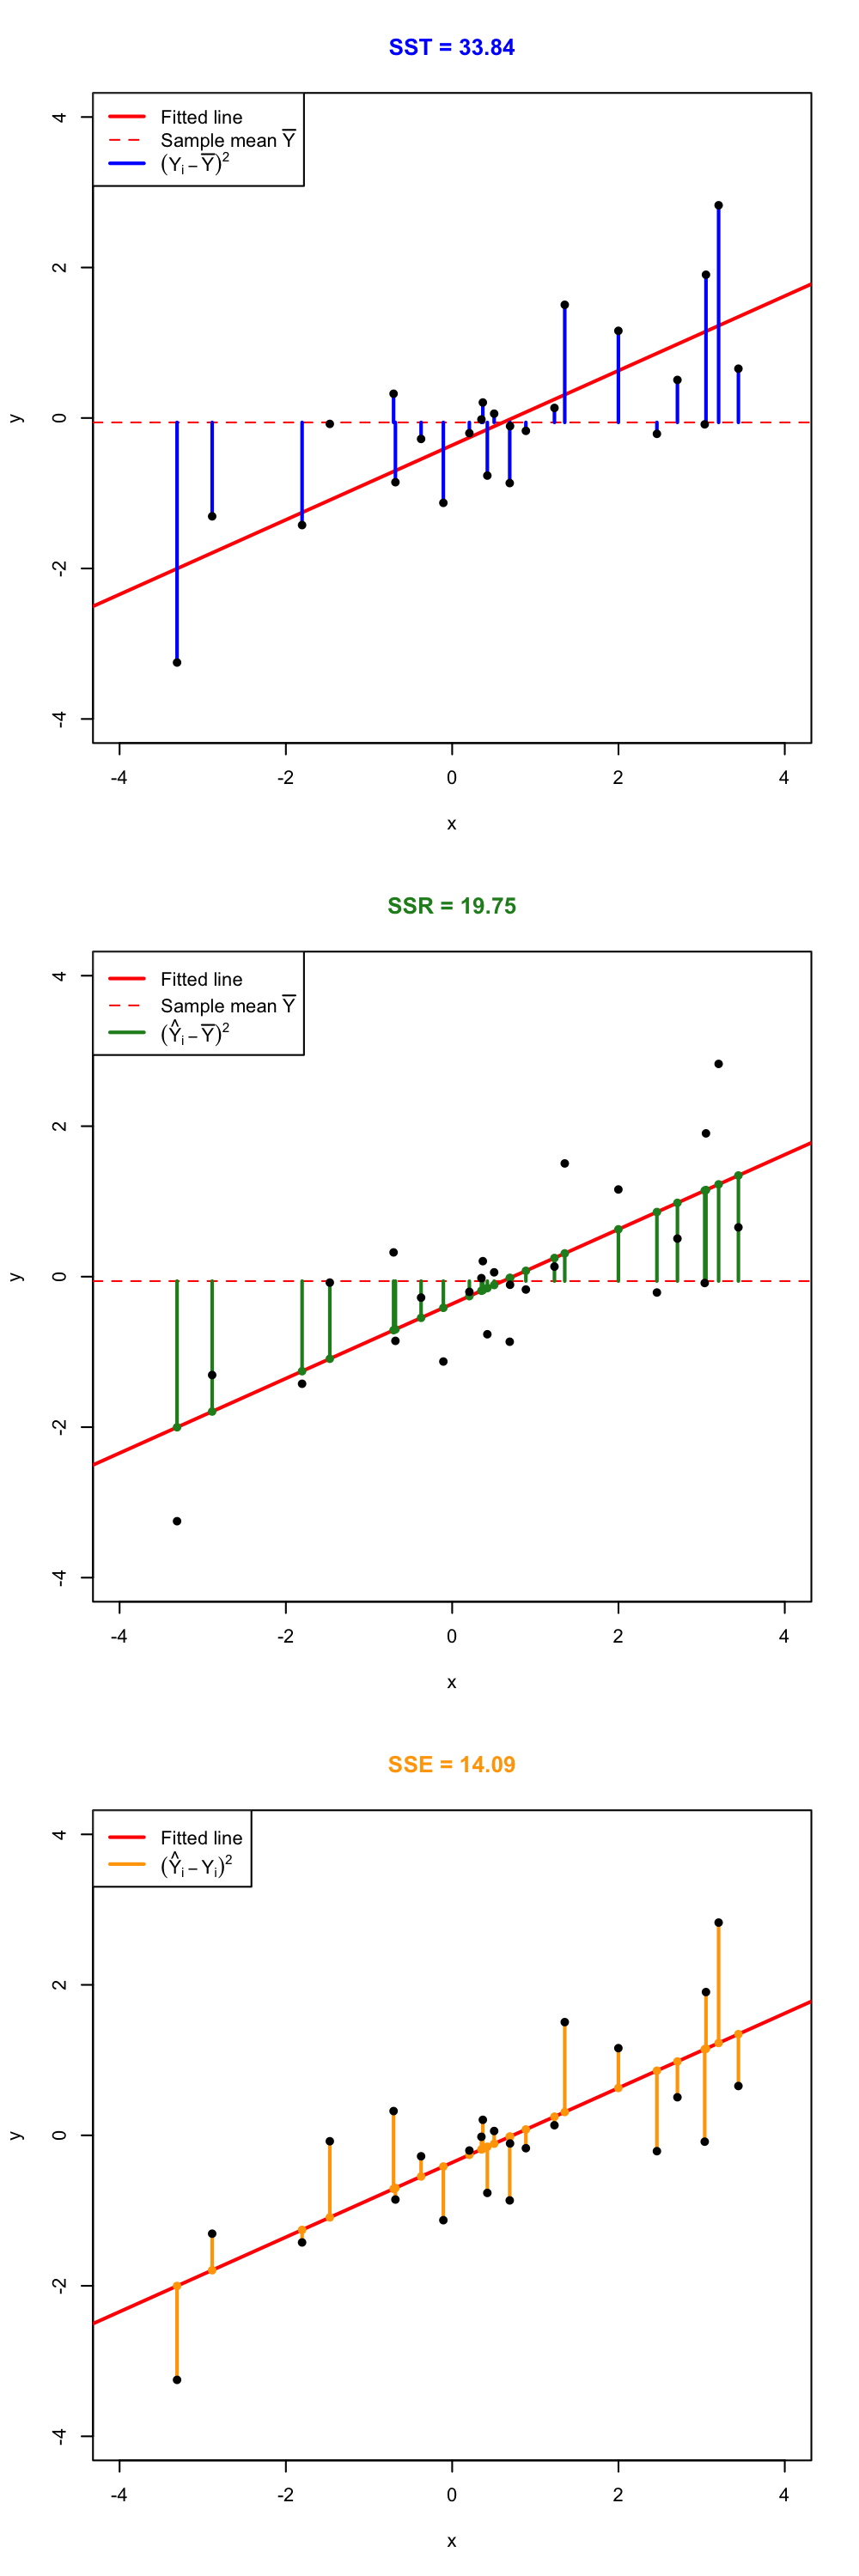
\includegraphics[width=0.7\linewidth]{img/anova} 

}

\caption{Visualization of the ANOVA decomposition. SST measures the variation of $Y_1,\ldots,Y_n$ with respect to $\bar Y$. SST measures the variation with respect to the conditional means, $\hat \beta_0+\hat\beta_1X_i$. SSE collects the variation of the residuals.}\label{fig:anova}
\end{figure}

\begin{rmdinsight}
Click here to see the ANOVA decomposition and its dependence on
\(\sigma^2\) and \(\hat\sigma^2\).'
\end{rmdinsight}

The ANOVA table summarizes the decomposition of the variance. Here is
given in the layout employed by \texttt{R}.

\begin{longtable}[]{@{}llllll@{}}
\toprule
& Degrees of freedom & Sum Squares & Mean Squares & \(F\)-value &
\(p\)-value\tabularnewline
\midrule
\endhead
Predictor & \(1\) & SSR & \(\frac{\text{SSR}}{1}\) &
\(\frac{\text{SSR}/1}{\text{SSE}/(n-2)}\) & \(p\)\tabularnewline
Residuals & \(n - 2\) & SSE & \(\frac{\text{SSE}}{n-2}\) &
&\tabularnewline
\bottomrule
\end{longtable}

The \texttt{anova} function in \texttt{R} takes a model as an input and
returns the ANOVA table.

The ``\(F\)-value'' of the ANOVA table represents the value of the
\(F\)-statistic \(\frac{\text{SSR}/1}{\text{SSE}/(n-2)}\). This
statistic is employed to test

\begin{align*}
H_0:\beta_1=0\quad\text{vs.}\quad H_1:\beta_1\neq 0,
\end{align*}

that is, the hypothesis of no linear dependence of \(Y\) on \(X\). The
result of this test is completely equivalent to the \(t\)-test for
\(\beta_1\) that we saw previously in the Hypothesis testing (this is
something \emph{specific for simple linear regression} -- the \(F\)-test
will not be equivalent to the \(t\)-test for \(\beta_1\) in the Mulitple
Linear Regression).

It happens that

\begin{align*}
F=\frac{\text{SSR}/1}{\text{SSE}/(n-2)}\stackrel{H_0}{\sim} F_{1,n-2},
\end{align*}

where \(F_{1,n-2}\) is the \emph{Snedecor's \(F\)
distribution}\footnote{The \(F_{n,m}\) distribution arises as the
  quotient of two independent random variables \(\chi^2_n\) and
  \(\chi^2_m\), \(\frac{\chi^2_n/n}{\chi^2_m/m}\).} with \(1\) and
\(n-2\) degrees of freedom.

If \(H_0\) is true, then \(F\) is expected to be \emph{small} since SSR
will be close to zero. The \(p\)-value of this test is the same as the
\(p\)-value of the \(t\)-test for \(H_0:\beta_1=0\).

\subsection{\texorpdfstring{The \(R^2\)
Statistic}{The R\^{}2 Statistic}}\label{the-r2-statistic}

To calculate \(R^2\), we use the formula

\[ R^2 = \frac{\text{TSS} - \text{RSS}}{\text{TSS}} = 1- \frac{\text{RSS}}{\text{TSS}} \]

where \(\text{TSS} = \sum (y_i - \bar{y})^2\) is the \emph{total sum of
squared}.

\(R^2\) measures the \emph{proportion of variability in} \(Y\)
\emph{that can be explained using} \(X\). An \(R^2\) statistic that is
close to 1 indicates that a large proportion of the variability in the
response has been explained by the regression. A number near 0 indicates
that the regression did not explain much of the variability in the
response; this might occur because the linear model is wrong, or the
inherent error \(\sigma^2\) is high, or both.

It can be shown that in this simple linear linear regression setting
that \(R^2 = r^2\), where \(r\) is the correlation between \(X\) and
\(Y\):

\[ r = \frac{cov(X,Y)}{\sigma_X \sigma_Y} \]

\begin{rmdcaution}
\(R^2\) does not measure the correctness of a linear model but its
\textbf{usefulness} (for prediction, for \emph{explaining the variance}
of \(Y\)), assuming the model is correct.

Trusting blindly the \(R^2\) can lead to catastrophic conclusions, since
the model may not be correct.
\end{rmdcaution}

So remember:

\begin{rmdinsight}
A large \(R^2\) means \emph{nothing} if the \textbf{assumptions of the
model do not hold}. \(R^2\) is the proportion of variance of \(Y\)
explained by \(X\), but, of course, \emph{only when the linear model is
correct}.
\end{rmdinsight}

◼


\end{document}
